	% Базовые настройки
\documentclass[a4paper,12pt]{report}
\usepackage[T2A]{fontenc}
\usepackage[utf8]{inputenc}
\usepackage[english,russian]{babel}
\usepackage{amssymb,amsfonts,amsmath,mathtext,cite,enumerate,float} 
\usepackage{graphicx}	% for pictures 
\usepackage{subcaption}	% for pictures
\usepackage[russian]{babel}
\captionsetup{justification=centering, labelfont=bf}
\usepackage{titlesec}
\usepackage{lipsum}
\graphicspath{{images/}}
\makeatletter
\renewcommand{\@biblabel}[1]{#1.}
\usepackage{indentfirst}
\makeatother
\usepackage{url}
\bibliographystyle{utf8gost71u}

% Поля страницы
\usepackage{geometry} 
\geometry{left=2cm}
\geometry{right=1.5cm}
\geometry{top=1cm}
\geometry{bottom=2cm}

% Страницы с номера 2
\setcounter{page}{1}  % Сбросить страницы
\renewcommand{\thepage}{\the\numexpr\value{page}+2}
\renewcommand{\thefigure}{\arabic{figure}}
\setcounter{figure}{1}

\begin{document}
\begin{titlepage}
\newpage

\begin{center}
Санкт-Петербургский государственный университет \\
\vspace{1cm}
Кафедра системного программирования \\*
Группа 22.Б11-мм \\*
\hrulefill
\end{center}

\vspace{8em}

\begin{center}
\Large \textbf{Разработка мобильного приложения для развития\\музыкальных навыков}
\end{center}

\vspace{2.5em}

\begin{center}
\LARGE \textsc{\textit{Зайцев Дмитрий Сергеевич }}
\end{center}

\begin{center}
\textsc{Отчёт по учебной практике}
\end{center}

\vspace{6em}

\begin{flushright}
Научный руководитель:\\
старший преподаватель СПбГУ Сартасов С. Ю.
\end{flushright}

\vspace{\fill}

\begin{center}
Санкт-Петербург\\2023
\end{center}

\end{titlepage} % титульный лист
\tableofcontents % это оглавление, которое генерируется автоматически
\chapter*{Введение}
\addcontentsline{toc}{chapter}{Введение}
\setlength\parindent{1.5em} 
\par 
Музыка всегда была одним из самых популярных видов искусств. Способность выражать мысли и чувства с помощью звука никогда не переставала интересовать человечество. Множество людей с самыми разными целями и подходами к обучению выбирали и продолжают выбирать музыку как объект для своего изучения. В наше время интерес к ней всё так же силён\cite{thamprasert2023network}.

Кроме того, по результатам проведённых исследований\cite{dumont2017music}, можно сделать вывод о том, что обучение музыке с ранних лет жизни способствует развитию у ребёнка:
\begin{itemize}
\item Памяти
\item Моторики
\item Внимания
\item Навыков коммуникации
\item Способности различать сложные эмоции и контролировать их
\item Навыков владения языком и речью
\end{itemize}\par
Что, безусловно, говорит о полезности прививания любви к данному виду творчества.\par

Изучение музыки - очень трудоёмкий процесс, требующий от человека не только желания погрузиться в новую область знаний, но и регулярных занятий, постоянной работы над ошибками, наличия рядом опытного преподавателя. Одним из важнейших элементов обучения является развитие \textit{музыкального слуха}, т.е. способности анализировать музыку без прямого чтения нот. Этот навык необходим как ученикам музыкальных школ для успешной сдачи экзаменов, так и людям, изучающим музыку самостоятельно.\par

Однако, несмотря на стремительное развитие технологий, на данный момент существует не так много эффективных решений для развитиях этих навыков, объединяющих в себе удобство и практичность.
\titleformat{\chapter}[display]
  {\normalfont\bfseries}{}{0pt}{\Huge}
\chapter{Задачи}

\textbf{Целью} работы является создание мобильного приложения, которое смогло бы облегчить процесс формирования способности определения интервалов на слух. \medskip\par
В ходе работы были поставлены следующие \textbf{задачи} на семестр:
\begin{enumerate}
\item сбор сведений о существующих решениях
\item их анализ и выявление потребностей пользователей
\item разработка требований к приложению на основании полученных данных
\item изучение необходимых технологий
\item разработка архитектуры, позволяющей перенести в приложения абстрактные музыкальные понятия
\item реализация библиотеки, содержащей необходимые для работы с музыкой объекты
\item реализация UI-составляющей приложения, разработка специальных стилей и компонентов
\item создание первого обучающего режима
\end{enumerate}\par
\chapter{Обзор}
\section{Анализ существующих решений}
Перед началом работы над приложением был проведён анализ существующих решений. Целью было выявление их преимуществ и недостатков, особенно важно было подчерпнуть удачные идеи, которые были бы полезны для пользователя. \par
В процессе сбора информации были рассмотрены наиболее информативные отзывы от пользователей на несколько приложений с наибольшим числом скачиваний. Ниже приведены результаты оценки каждого из приложений.
% ---
\subsection[Absolute ear]{Absolute ear\cite{Apps1}}
\begin{minipage}[t]{0.45\textwidth}
\textbf{Достоинства:}
\begin{itemize}
  \item[+] Есть раздел с теорией, интегрированный в обучение;
  \item[+] Большое количество упражнений;
  \item[+] Оценка и поощрение достижений пользователя, дополнительная мотивация к зантиям;
  \item[+] Возможность просмотра статистики и выявления слабых мест.
\end{itemize}
\end{minipage}
\hfill
\begin{minipage}[t]{0.45\textwidth}
\textbf{Недостатки:}
\begin{itemize}
  \item[-] Возможны баги, при которых результат пользователя оценивается некорректно;
  \item[-] Интерфейс не уведомляет пользователя об ошибках;
  \item[-] Интерфейс ориентирован только на знающих терминологию людей;
  \item[-] Почти полностью отсутствует возможность настройки упражнений.
\end{itemize}
\end{minipage} 
% ---
\subsection[Functional Ear Trainer]{Functional Ear Trainer\cite{Apps2}}
\begin{minipage}[t]{0.45\textwidth}
\textbf{Достоинства:}
\begin{itemize}
  \item[+] Есть режим с полной настройкой упражнения;
  \item[+] Интерфейс адаптирован под всех пользователей (разные форматы отображения информации);
  \item[+] Большое количество настроек как интерфейса, так и всего остального.
\end{itemize}
\end{minipage}
\hfill
\begin{minipage}[t]{0.45\textwidth}
\textbf{Недостатки:}
\begin{itemize}
  \item[-] Музыкальные обозначения не подходят для всех пользователей (в России они другие);
  \item[-] Упражнения не учитывают предыдущие попытки пользователя, возможны повторения;
  \item[-] Из-за платной подписки урезан основной контент.
\end{itemize}
\end{minipage}
% ---
\subsection[My Ear Trainer]{My Ear Trainer\cite{Apps3}}
\begin{minipage}[t]{0.45\textwidth}
\textbf{Достоинства:}
\begin{itemize}
  \item[+] Уникальный режим - подбор целой мелодии на слух;
  \item[+] Большое разнообразие упражнений и выбор сложности для каждого;
  \item[+] Есть курсы с введением в теорию.
\end{itemize}
\end{minipage}
\hfill
\begin{minipage}[t]{0.45\textwidth}
\textbf{Недостатки:}
\begin{itemize}
  \item[-] Почти нет настроек интерфейса под разных пользователей;
  \item[-] Нет поддержки некоторых языков и их обозначений.
\end{itemize}
\end{minipage}
\subsection{Результаты анализа}
Исходя из приведённого выше обзора, можно сделать вывод, что на данный момент уже существует несколько решений для представленной проблемы. Это говорит о присутствии реальной потребности в приложениях, помогающих в освоении музыкальных навыков.\par
В то же время, ни одно из них полностью не решает проблемы. Почти в каждом приложении основной контент доступен лишь по подписке, интерфейс не адаптирован под пользователей с разными знаниями, иногда допускаются грубые ошибки при подборе или проверке заданий, доступно очень маленькое количество настроек как пользовательского интерфейса, так и самих упражнений. Более того, для русских пользователей, желающих учиться по принятым в нашей стране обозначениям, круг выбора сводится всего до нескольких вариантов.\par
Однако, при разработке представленных аналогов было реализовано множество хороших решений, которые следовало бы особо отметить: большое разнообразие различных упражнений с разделением на уровни сложности, есть возможность осваивать теорию (словари с терминами, статьи) и параллельно закреплять знания на практике, почти во всех приложениях ведётся анализ достижений пользователя и сбор статистики. Также одна из интересных функций - режим, где возможна полная настройка занятия (представлено лишь в \textit{Functional Ear Trainer}, но по отзывам многим это нужно).
\section{Требования к приложению}
Исходя из результатов проведённого анализа, были сформулированы \textbf{требования}. Обучающее приложение должно: 
\begin{enumerate}
\item запускаться на устройствах под управлением ОС Android;
\item быть удобным в использовании как для людей, владеющих музыкальной терминологией и нотной грамотой, так и для новичков;
\item оценивать результаты пользователя, поощряя его за новые свершения, например возможность просмотра статистики, получения “достижений” (как вариант);
\item поддерживать возможность создавать расписание занятий и получать уведомления в запланированное для них время;
\item позволять использовать реальный инструмент как способ ввода информации для прохождения заданий;
\item иметь разнообразные упражнения для развитиях слуха с возможностью настройки сложности;
\item поддерживать разные языки и обозначения.
\end{enumerate}\par
\section{Используемые технологии}
Основными критериями выбора языка программирования были: возможность запускать код на телефонах под управлением Android, наличие удобных инструментов для мобильной разрабоки (как библиотек и платформ, так и IDE) и удобный синтаксис. Исходя из этих критериев, для написания приложения был выбран \textbf{Kotlin}.\par
Kotlin на данный момент является одним из самых быстроразвивающихся языков программирования\cite{Github}. Кроме этого, он исполняется в \emph{JVM} и имеет совместимость с Java-кодом, что невероятно полезно, так как за всё время их существования, накопилось огромное количество библиотек, платформ и прочих готовых решений для часто встречающихся проблем. Ещё одним преимуществом является поддержка Kotlin в одной из самых популярных IDE для мобильной разработки - \emph{Android Studio}, ведь она позволяет значительно ускорить все этапы разработки продукта. Наличие у Kotlin понятного и удобного синтаксиса стало решающей причиной выбрать этот язык для разработки.\par
В качестве системы сборки проекта был выбран \textbf{Gradle}, в основном из-за быстрой сборки многомодульных приложений и удобстве в настройке.\par
Фреймворк \textbf{JUnit5}, предназначенный для написания тестов под JVM, является одним их самых популярных решений. Он приятен в использовании и имеет хорошую документацию, за что и был выбран.\par
Одним из самых важных аспектов разработки ПО является создание практичного и красивого пользователю интерфейса. Для этих целей идеально подходит платформа \textbf{Jetpack Compose}. Он позволяет создавать интерфейс с помощью коротких конструкций кода на Kotlin, имеет низкий порог вхождения, но при этом даёт возможность создавать современный интерфейс.

\chapter{Реализация}
\section{Архитектура}
Ещё на этапе планирования архитектуры приложения было принято решение выделить для логики, связанной с музыкой, отдельный модуль. На данный момент все классы, представляющие собой ключевые музыкальные абстракции (такие как: нота, мелодия, длительность и т.д.), находятся в модуле \textbf{MusicLib}. Во втором модуле (\textbf{App}) содержатся UI-компоненты и некоторые классы, позволяющие связывать пользовательский интерфейс и классы из MusicLib. Благодаря такому разделению появляется возможность гораздо проще проводить тестирование и логически отделять разные абстракции друг от друга.\par
Для представления главных музыкальных абстракций на данный момент существует несколько классов: \textit{Interval}, \textit{NoteRange}, \textit{Melody}, \textit{Note}, \textit{Pause} и \textit{MelodyNote}. Для хранения мелодии применяется класс \textit{Melody}, а для её построения необходима последовательность из нот (\textit{MelodyNote}), либо музыкальных пауз. При этом важным является тот факт, что для представления ноты было принято решение сделать сразу два класса, главное их отличие в том, что \textit{Note} представляет собой просто звук определённой высоты, а \textit{MelodyNote} содержит дополнительные свойства, позволяющие более детально управлять звуком. Классы \textit{NoteRange} и \textit{Interval} представляют собой соответственно диапазон нот (например, для фортепиано) и музыкальный интервал (расстояние между звуками). Кроме этого, существует также множество классов и перечислений для описания различных музыкальных свойств.\par
Модуль App содержит реализацию классов, связывающих описанные выше классы и интерфейс, доступный пользователю. На данный момент реализована возможность создавать свои виртуальные инструменты с помощью наследования от класса \textit{AbstractInstrument} и возможность извлекать из них звуки соответствующих инструментов с помощью \textit{MelodyPlayer}.\par
Было реализованно также и несколько ключевых элементов интерфейса. Например, класс \textit{PianoKeyboard} позволяет отрисовывать на экране клавиатуру переданных размеров и с указанным диапазоном клавиш. Этот элемент полезен как для пользователей, не имеющих реального инструмента, так и для интерфейса некоторых заданий.

\begin{figure}[H]
  \centering
  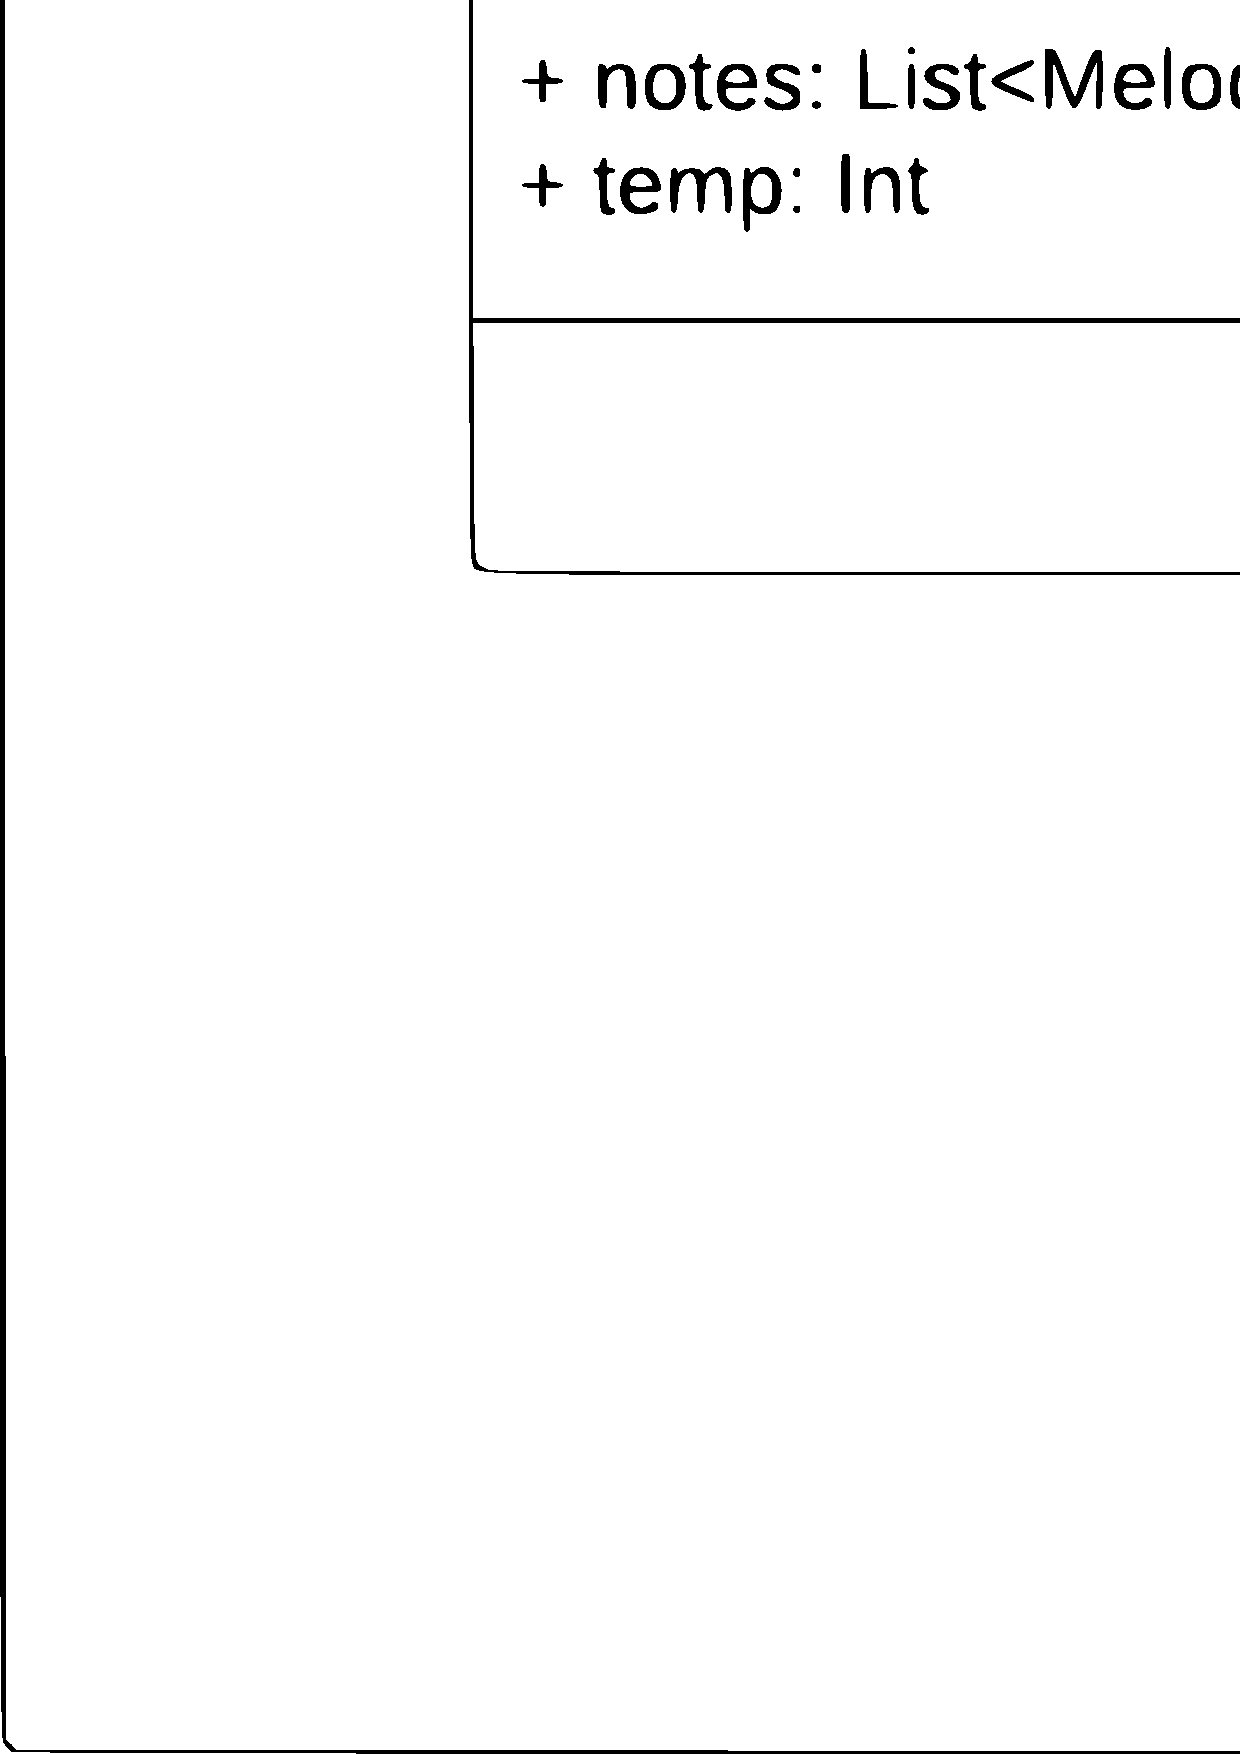
\includegraphics[width=\linewidth]{UML.pdf}
  \caption{UML-диаграмма библиотеки.}
  \label{fig:boat1}
\end{figure}

\section{Интерфейс приложения}
Главными требованиями к пользовательскому интерфейсу были: удобство в пользовании для людей, не знакомых со сложными обозначениями и терминами, современный дизайн, поддержка разных языков. Важно было учесть, что основные пользователи приложения (учащиеся музыкальных школ) также требуют особого подхода, так как сложный и перегруженный деталями интерфейс может отвлекать ребёнка и затруднять понимание материала.\par 
Цветовая палитра приложения(рис. \ref{fig:colors}) была специально подобрана так, чтобы не отвлекать от упражнений. Цвета приглушены, но при этом хорошо сочетаются друг с другом.\par

\begin{figure}[H]
  \centering
  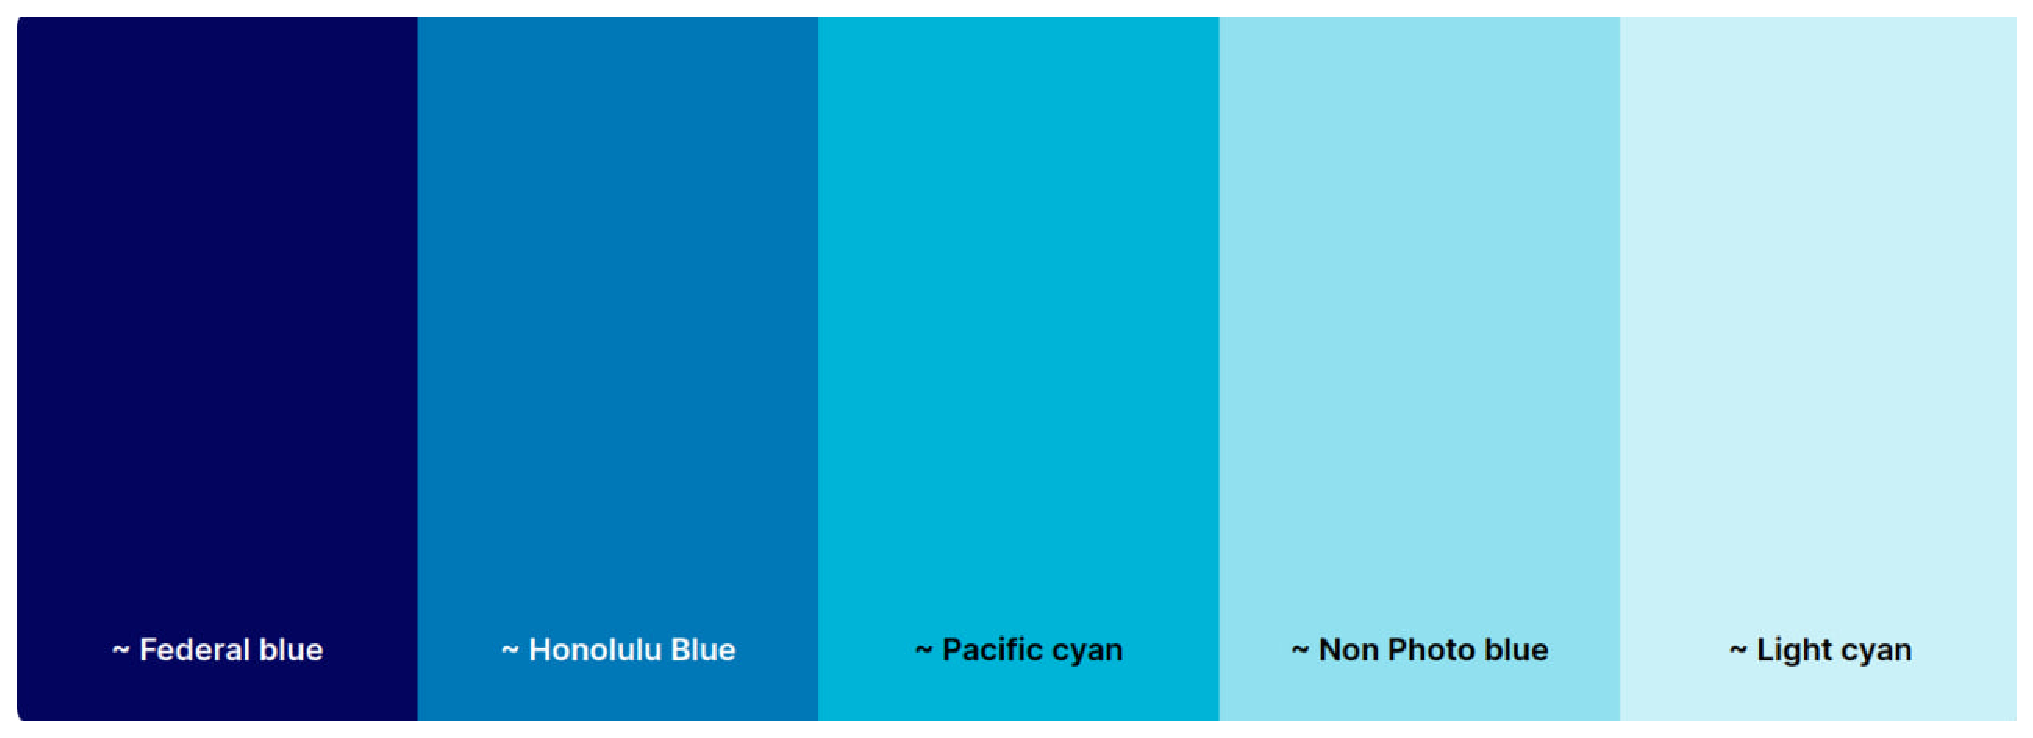
\includegraphics[width=0.5\linewidth]{colors.eps}
  \caption{Цветовая палитра приложения}
  \label{fig:colors}
\end{figure}

Формы элементов интерфейса также подбирались исходя из предположений о том, что обилие углов и деталей будет отвлекать и слишком бросаться в глаза. Было создано несколько дополнительных форм и анимаций для специальных элементов, так как подходящих в наборе Jetpack Compose найти не удалось.\par

\begin{figure}[H]
  \centering
  \begin{subfigure}[b]{0.35\linewidth}
    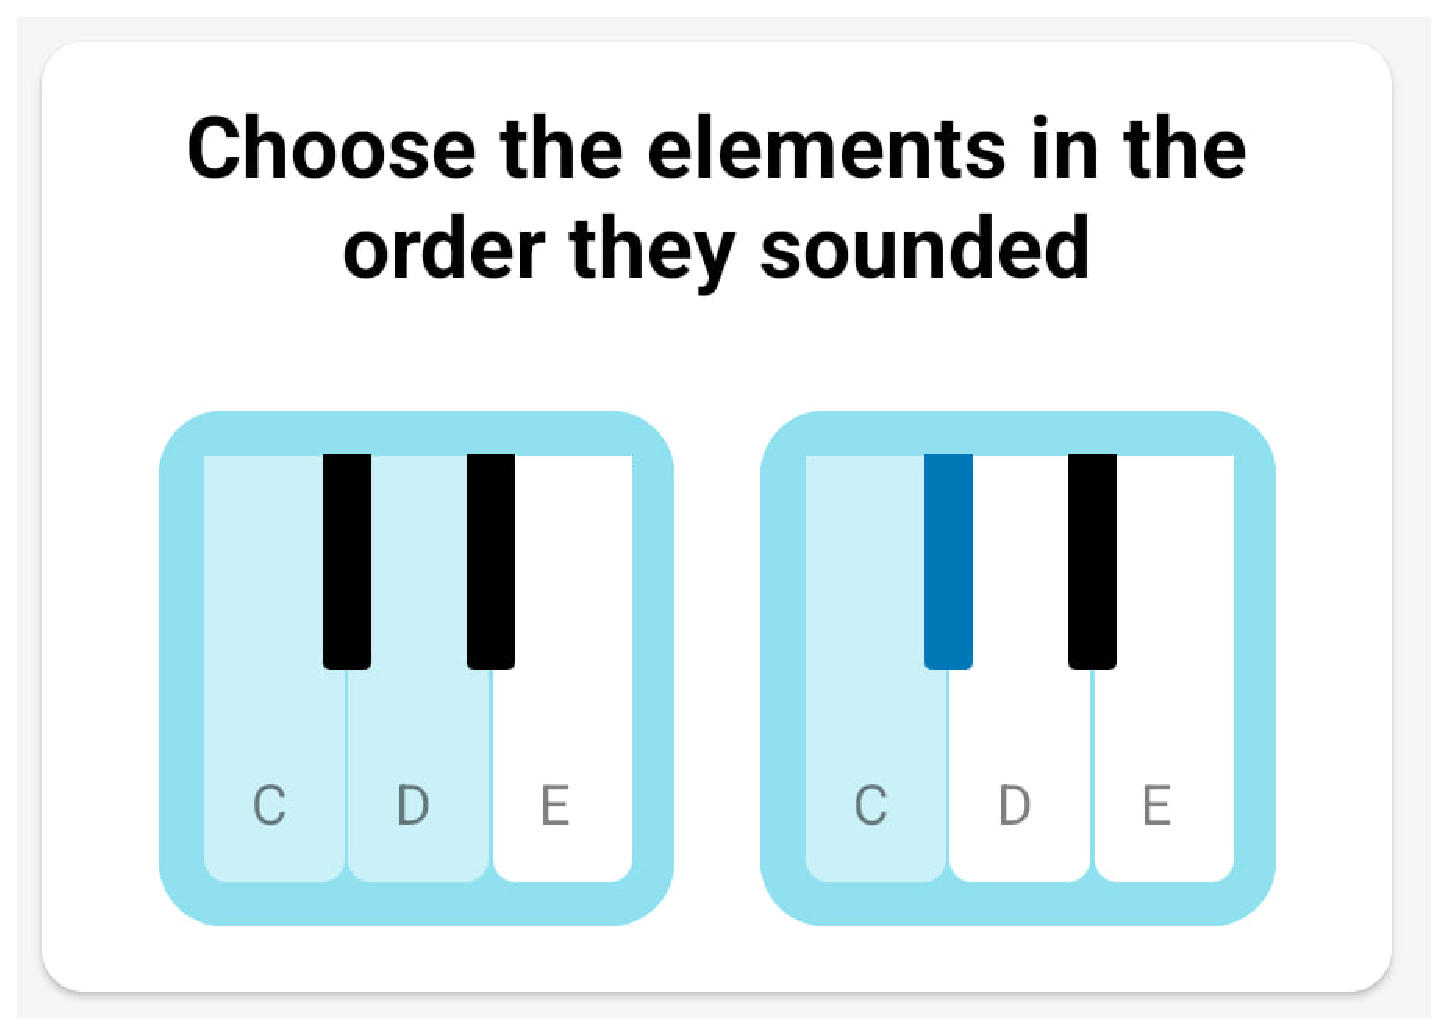
\includegraphics[width=\linewidth]{example1.eps}
    \caption{Piano Checkbox.}
  \end{subfigure}
  \begin{subfigure}[b]{0.4\linewidth}
    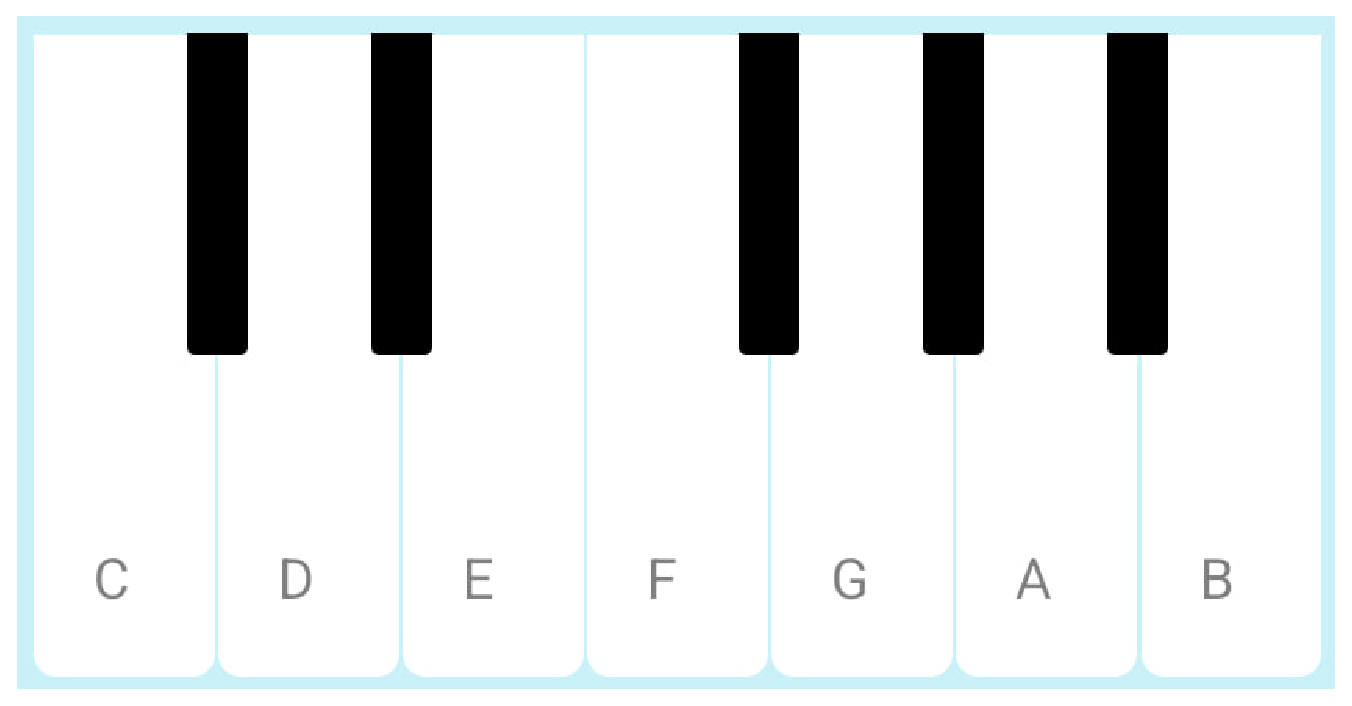
\includegraphics[width=\linewidth]{example4.eps}
    \caption{Piano Keyboard.}
  \end{subfigure}
  \begin{subfigure}[b]{0.4\linewidth}
    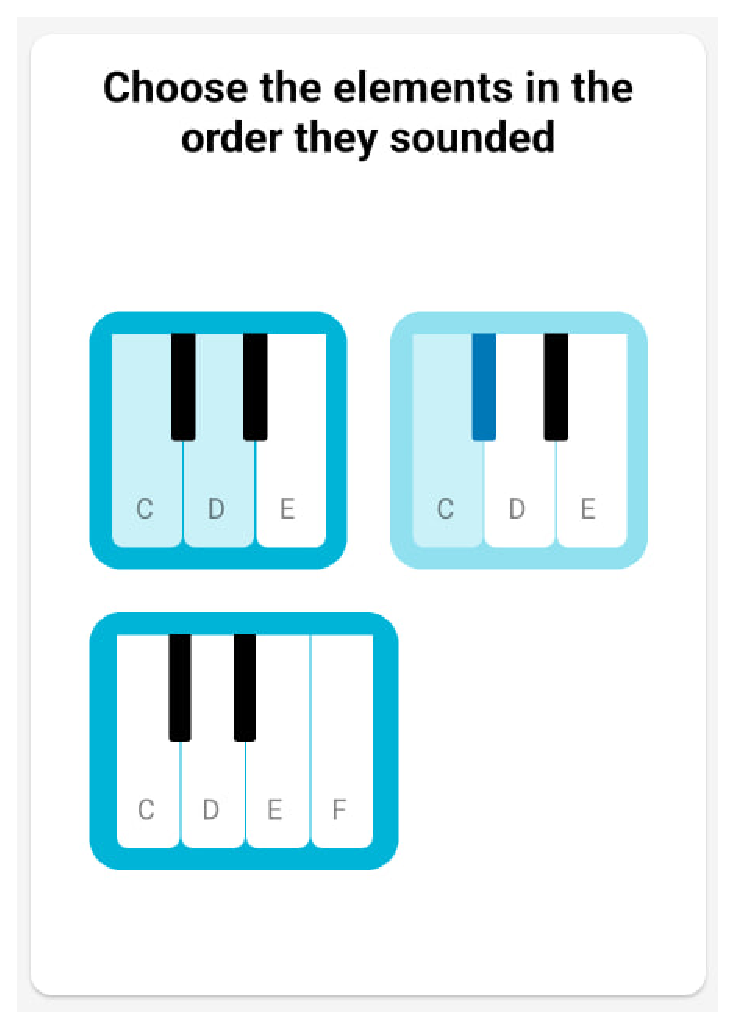
\includegraphics[width=\linewidth]{example2.eps}
    \caption{Piano Checkbox (с выбранными вариантами).}
  \end{subfigure}
    \begin{subfigure}[b]{0.3\linewidth}
    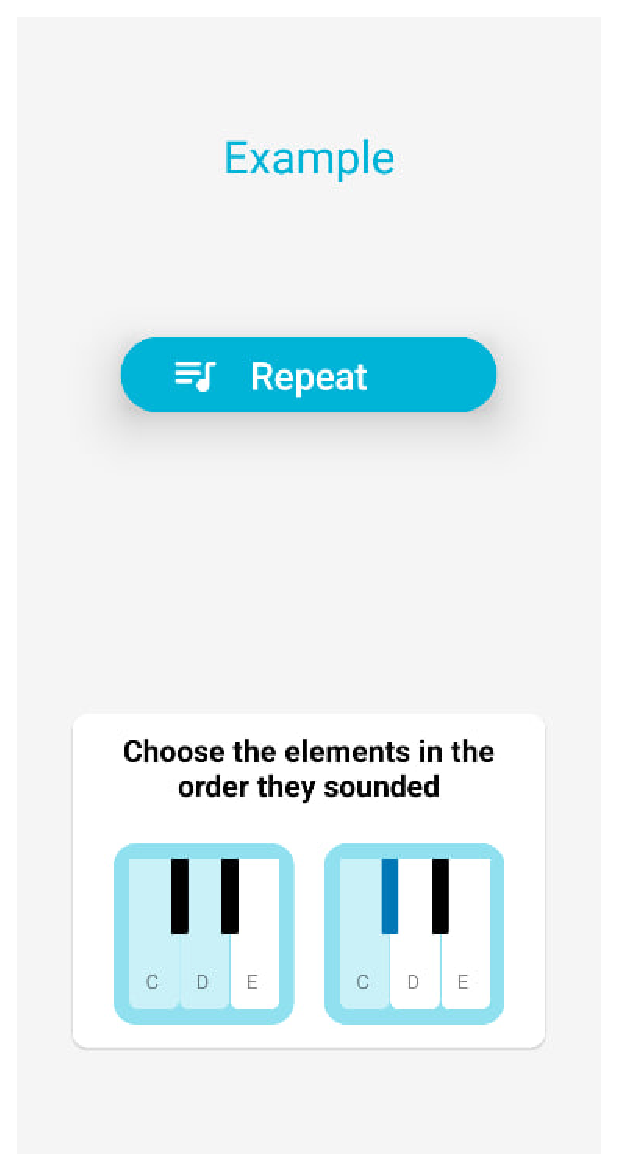
\includegraphics[width=\linewidth]{example3.eps}
    \caption{Примерный вид упражнения.}
  \end{subfigure}
  \caption{Основные элементы пользовательского интерфейса.}
  \label{fig:app}
\end{figure}
\bibliography{biblio/lit}
\end{document}